% main.tex — EMA-Det, Springer SIVP extended journal draft
%
% STATUS: content draft. \documentclass is a standard `article` placeholder —
% swap to Springer Nature's `sn-jnl.cls` (obtained from the SIVP submission
% portal, not fetched here) before submission; section structure and
% \maketitle metadata below are written to match sn-jnl.cls's expected
% \title/\author/\abstract/\keywords commands as closely as a placeholder
% class allows, but double-check against the actual class's documentation.
%
% All numeric results below come from this repository's own reproduction
% (see ../results/controlled_comparison.json, ../results/pr_curve.json,
% ../results/onnx_benchmark_*.json) — nothing here is carried over from the
% conference draft without being re-verified.
%
% OPEN ITEMS (do not submit before resolving):
%   - Table III's MobileNetV3-Small / ShuffleNetV2 / YOLOv8n rows: training
%     in progress at draft time, marked TODO below.
%   - Section "Cross-Sensor Generalization" from the original Faz 1 plan:
%     no thermal/IR dataset is available in this project; either source one
%     or drop the claim. Not fabricated here.
%   - Section "Hardware Validation": FPGA synthesis has not been run (no
%     Vivado/Vitis HLS toolchain in the dev environment) — written to
%     describe only what is actually true (C++ translation + real-weight
%     numerical validation prepared, not yet synthesized) plus the ONNX/CPU-
%     GPU proxy latency numbers, clearly labeled as not Jetson/FPGA.
%   - Author affiliations, funding/acknowledgment text, and any SIU-paper
%     copyright/permission language needed for a journal extension: left as
%     placeholders for the authors to fill in directly.

\documentclass[12pt]{article}
\usepackage[utf8]{inputenc}
\usepackage[T1]{fontenc}
\usepackage{graphicx}
\usepackage{amsmath,amssymb}
\usepackage{booktabs}
\usepackage{hyperref}
\usepackage{geometry}
\geometry{margin=1in}

\title{EMA-Det: Hardware-Aware Edge Verification for Two-Stage UAV Detection}

\author{
Enes Mert Ayd{\i}n \and Osman Toklu{\u{g}}lu \and Enver {\c{C}}avu{\c{s}} \\
\small Department of Electrical and Electronics Engineering, Ankara Y{\i}ld{\i}r{\i}m Beyaz{\i}t University, Ankara, T{\"u}rkiye
}
\date{}

\begin{document}
\maketitle

\begin{abstract}
Autonomous detection of Low-Slow-Small (LSS) UAVs on edge devices necessitates
two-stage pipelines, in which a lightweight proposal stage nominates
candidate regions that a verification network must confirm or reject under
tight compute and memory budgets. This paper presents EMA-Det, a
hardware-aware region-verification network combining a physically
initialized (Laplacian/Sobel) first layer with two early-exit gates that let
confidently-background candidates skip the majority of the network. We
identify and correct two methodological issues present in our earlier
conference report: (i) a confound between an attention-module (CBAM)
ablation and the main comparison table, caused by the two being trained
under different budgets, and (ii) train/test leakage in the region-patch
dataset, traced to near-duplicate raw source photographs (consistent with
sequential video-frame extraction) being split at the patch level rather
than the source-photograph level. Correcting both, we retrain EMA-Det with
and without CBAM under an identical $N=5$-seed, 150-epoch protocol on a
deduplicated, source-level-split dataset. The corrected results show CBAM
improves point-estimate localization quality (mAP@0.5:0.95: $28.93\pm1.67\%$
vs.\ $25.18\pm2.08\%$) but nearly quadruples recall's run-to-run standard
deviation ($8.85$ vs.\ $2.54$ points, with 2 of 5 seeds collapsing to
74--79\% recall) — an unacceptable reliability profile for a
safety-relevant edge verifier, and the actual reason CBAM is excluded from
the final architecture, rather than a uniform accuracy penalty as our
preliminary ablation had suggested. \emph{[Abstract to be finalized once
Table III's additional lightweight-model comparisons complete — see TODO in
source.]}
\end{abstract}

\noindent\textbf{Keywords:} UAV Detection, Edge Computing, Region
Verification, Early-Exit, Hardware-Aware Design, Reproducibility


\section{Introduction}

Asymmetric threats posed by Low-Slow-Small (LSS) class Unmanned Aerial
Vehicles (UAVs) to civilian and military critical infrastructure require an
extremely fast and reliable ``sense-decide-act'' loop in modern autonomous
air-defense systems~\cite{luo2021threat}. Electro-optical (EO) sensors today
are typically 4K ($3840\times2160$) or higher resolution; processing such
high-resolution video streams directly and in full-frame on edge devices
using standard deep CNNs is infeasible in real time due to bandwidth and
memory constraints~\cite{qasaimeh2019comparing}.

To alleviate this pixel load, fielded autonomous systems typically use a
two-stage cascade~\cite{fouda2022lightweight}. A first stage (radar priors,
acoustic sensors, or simple motion/background-subtraction algorithms)
identifies candidate Regions of Interest (RoI) in the frame. A second stage
crops these small patches (commonly $64\times64$ or $128\times128$ pixels)
and feeds them to a neural network for verification.

Prior work in this space commonly adapts general-purpose detectors (the
YOLO family, SSD) to the RoI-verification
task~\cite{achmadiah2025energy,cao2023improved}. We argue, and demonstrate
empirically, that RoI verification in a two-stage system is \emph{not}
simply a scaled-down detection problem. On edge devices, memory bandwidth is
a more critical bottleneck than raw compute (GFLOPs)~\cite{qasaimeh2019comparing};
even edge-compressed YOLO variants (e.g.\ YOLO-Nano) run into resource
limits and energy--performance bottlenecks on FPGA-class
hardware~\cite{adiono2021low}. Architectures designed for full-frame
operation, compressed into a micro-input regime, suffer spatial feature loss
from their deep global-pooling stages and asymmetric data flow.

Since total system recall in a two-stage architecture is
$R_{\text{total}} = R_{\text{proposal}} \times R_{\text{verifier}}$, a
verifier's false negative is a system-level miss. This makes recall, not
mAP, the design-critical metric for the second stage.

\paragraph{Contributions.} (1) We formalize the RoI-verification problem in
two-stage systems and show empirically that full-frame attention mechanisms
degrade target features in the micro-input regime — with the important
caveat, corrected in this extended version, that the effect is on
\emph{training stability} rather than a uniform accuracy penalty (Section~
\ref{sec:cbam}). (2) We convert the asymmetric background distribution of
candidate regions (mostly empty sky) into a latency advantage via an
early-exit mechanism. (3) We identify and correct a train/test leakage bug
in the RoI dataset construction pipeline that inflated our own preliminary
results, and release the corrected dataset-construction methodology.
(4) We present a controlled, $N=5$-seed comparison — the conference
version's ablation and main results tables were produced under different
training budgets, which this version corrects.


\section{EMA-Det: Architecture and Method}

\subsection{System-Level Latency Model}
In a two-stage architecture, total system latency $T_{\text{total}}$ is
modeled as the proposal time plus the sum of per-candidate verification
times (Eq.~\ref{eq:latency}).
\begin{equation}
T_{\text{total}} = T_{\text{proposal}} + \sum_{i=1}^{N_{\text{RoI}}} T_{\text{verifier}}^{(i)}
\label{eq:latency}
\end{equation}
When a general-purpose full-frame detector is used as the verifier, every
candidate patch — including empty-sky patches — pays the full network's
fixed cost. EMA-Det's dynamic early-exit structure converts this linear
scaling into an asymptotic one.

\subsection{Laplacian/Sobel-Initialized Kernel Bank}
At a constrained $128\times128$ resolution, small targets carry limited
spatial information. Standard Xavier/Kaiming random initialization requires
the network to learn edge boundaries from scratch, increasing iteration cost
and training variance. The first convolution layer's weights $W_1$ are
instead initialized from a deterministic bank of Laplacian ($L$)
\cite{marr1980theory} and Sobel ($S$) \cite{kanopoulos1988design} operators:
\begin{equation}
W^{(0)}_{1,c} = \begin{cases}
K_c, & c \in \{1,\dots,K\} \\
R_c, & c \in \{K+1,\dots,C_{\text{out}}\}
\end{cases}
\label{eq:init}
\end{equation}
where $K_c$ are the deterministic physical priors ($L$, $L_2$, $S_x$, $S_y$,
and their signed sums) and $R_c \sim \mathcal{N}(0, 0.1)$ preserves the
layer's capacity to generalize beyond the fixed operators. These weights are
left unfrozen and are updated during training like any other layer (see
\texttt{ema\_det.py}'s self-test, which verifies both the initial values and
that gradients reach this layer).

\subsection{Architecture}
Figure~\ref{fig:arch} shows the network. Block~1 (Section 2.2) reduces
$1\times128\times128$ to $16\times64\times64$; Blocks~2--4 progressively
reduce to $128\times8\times8$; Block~5 fuses two parallel dilated branches
($d{=}1,2$) to $128\times4\times4$; Block~6 expands to $256\times4\times4$;
a verification head (global average pool, dropout $0.4$) produces a
classification logit and a 4-coordinate bounding-box refinement.

CBAM~\cite{woo2018cbam} was evaluated during architecture development and is
\emph{not} part of the default forward path — Section~\ref{sec:cbam}
presents the corrected, controlled evidence for that decision, which differs
qualitatively from the conference version's ablation.

\begin{figure}[t]
\centering
% \includegraphics[width=0.7\textwidth]{figures/architecture.pdf}
\caption{EMA-Det architecture. Dashed orange paths indicate early-exit
routes; candidates confidently classified as background at Gate~1 or
Gate~2 skip the remaining blocks.}
\label{fig:arch}
\end{figure}

\subsection{Loss Function}
The verification head is optimized with a combined classification and
box-regression loss (Eq.~\ref{eq:loss}):
\begin{equation}
\mathcal{L}_{\text{total}} = \lambda_{\text{cls}}\mathcal{L}_{\text{BCE}}(\hat{p}, p) + \lambda_{\text{box}}\mathcal{L}_{\text{CIoU}}(\hat{b}, b)
\label{eq:loss}
\end{equation}
where $\mathcal{L}_{\text{CIoU}}$ is the Complete-IoU loss~\cite{zheng2020distance},
with $\lambda_{\text{cls}}=1.0$. \textbf{Correction:} the conference draft
stated $\lambda_{\text{box}}=2.5$; the value actually used throughout
training and every ablation (verified directly in the training code) is
$\lambda_{\text{box}}=2.0$. This document uses the code-verified value.
Early-exit gates are supervised with their own BCE terms
($\lambda_{\text{gate1}}=0.3$, $\lambda_{\text{gate2}}=0.4$) against the
same binary label as the main head.

\subsection{Dynamic Early-Exit Gates}
Gates~1 and~2 (after Blocks~2 and~4) implement the asymptotic rule of
Eq.~\ref{eq:gate}: a candidate halts (classified background, no box
refinement) once its confidence falls below $1-\tau$; otherwise it proceeds.
\begin{equation}
\text{Result} = \begin{cases}
\text{Background (halt)}, & \hat{y}_i \le (1-\tau) \\
C_{i+1}(F_i)\ (\text{continue}), & \hat{y}_i > (1-\tau)
\end{cases}
\label{eq:gate}
\end{equation}


\section{Experimental Setup}

\subsection{Dataset Construction and a Corrected Leakage Bug}
\label{sec:leakage}

The dataset is built from three raw sources: rotary-wing and fixed-wing UAV
photographs (labeled) and empty-sky photographs (unlabeled, hard-negative
source). \textbf{This extended version corrects a train/test leakage bug
found in the conference version's dataset-construction script.}

The original pipeline cropped one positive patch (around each labeled UAV,
with a $3\times$ context factor) and one hard-negative patch (from the same
photograph, near but not overlapping the UAV) per raw image, then pooled
\emph{all} resulting patches from \emph{all} raw photographs and split them
into train/val/test by random shuffle at the \emph{patch} level. Two
problems compound here. First, the raw photograph pool itself was heavily
duplicated: an 8$\times$8 average-hash comparison found 52.1\% of raw
labeled-candidate photographs (and 69.1\% of raw sky photographs) have a
bit-identical near-duplicate elsewhere in the same pool — consistent with
sequential video-frame extraction (e.g.\ \texttt{rotor/0032.jpg} and
\texttt{rotor/0033.jpg} hash identically). Second, because splitting
happened at the patch level with no deduplication, near-duplicate source
photographs — and even sibling patches cropped from the very same
photograph — could land on opposite sides of the train/test boundary.
Empirically, 83.8\% of test-set positive (UAV) patches were bit-identical
to a training-set positive patch under the same hash.

We fix this in two steps, implemented in
\texttt{build\_dataset\_clean.py}: (1) deduplicate raw photographs via the
same average-hash (Hamming distance $\le 5$ clustered via union-find, one
representative kept per cluster, preferring a labeled member), reducing
5{,}921 raw labeled-candidate photographs to 2{,}142 unique ones (and 2{,}872
raw sky photographs to 887); (2) split the \emph{deduplicated photograph
pool} into train/val/test (70/15/15) \emph{before} any patch cropping, so
every patch derived from a given photograph is guaranteed to land in that
photograph's assigned split. Re-running the leakage check on the resulting
dataset finds the test-positive exact-duplicate rate drops from 83.8\% to
0.6\% (residual consistent with hash collisions on low-detail images, not
real duplication). As a direct consequence of removing duplicated content,
the dataset shrinks from 23{,}620 patches to 4{,}136 genuinely unique
patches (2{,}842 train / 662 val / 632 test).

We report all results in this paper on this corrected dataset. Numbers are
consequently not directly comparable to the conference version, which
reported inflated metrics due to leakage.

\subsection{Training Protocol}
All models are trained with AdamW, 5-epoch linear warmup followed by cosine
annealing, batch size 16, gradient clipping at norm 5.0. \textbf{Correction:}
the conference draft stated weight decay $=0.01$; the code-verified value
used throughout is $\text{weight\_decay}=10^{-4}$, which is what this
document uses. Early stopping uses patience 20 on validation mAP@0.5, for
up to 150 epochs. \textbf{All reported results use $N=5$ seeds
$\{42, 7, 123, 2024, 31415\}$ under this identical protocol} — including the
CBAM ablation, which in the conference version was run at a much smaller
budget ($N=1$, 50 epochs) than the main comparison table, confounding the
effect of CBAM with the effect of training budget. This version removes
that confound.

Augmentation excludes Mosaic/MixUp (destroys small-target shape at
$128\times128$); we use horizontal flip, brightness/contrast jitter,
directional motion blur, Gaussian noise, small-angle rotation, and coarse
dropout.


\section{Results}

\subsection{CBAM: A Stability Trade-off, Not a Uniform Penalty}
\label{sec:cbam}

Table~\ref{tab:cbam} reports the corrected, controlled $N=5$ comparison.

\begin{table}[t]
\centering
\caption{Controlled comparison, identical $N{=}5$-seed / 150-epoch / early-stopping(patience=20) protocol. Mean $\pm$ std over 5 seeds, clean test set.}
\label{tab:cbam}
\begin{tabular}{lccccccc}
\toprule
Config & mAP@0.5 & mAP@0.75 & mAP@.5:.95 & Precision & Recall & F1 & Mean IoU \\
\midrule
EMA-Det (final) & $56.64{\pm}2.44$ & $18.33{\pm}2.67$ & $25.18{\pm}2.08$ & $94.03{\pm}1.51$ & $\mathbf{96.33{\pm}2.54}$ & $\mathbf{95.14{\pm}1.51}$ & $62.53{\pm}1.45$ \\
EMA-Det + CBAM & $\mathbf{60.70{\pm}2.98}$ & $\mathbf{23.88{\pm}2.29}$ & $\mathbf{28.93{\pm}1.67}$ & $\mathbf{96.79{\pm}0.89}$ & $87.28{\pm}\mathbf{8.85}$ & $91.51{\pm}4.70$ & $\mathbf{66.43{\pm}0.88}$ \\
\bottomrule
\end{tabular}
\end{table}

This is qualitatively different from the conference draft's claim. CBAM
does \emph{not} uniformly degrade this architecture: point-estimate mAP,
mAP@0.75, mAP@0.5:0.95, precision, and mean IoU are all \emph{higher} with
CBAM. What breaks is reliability across random seeds: CBAM's recall standard
deviation ($8.85$ points) is $3.5\times$ EMA-Det-final's ($2.54$ points), driven
by 2 of 5 seeds (7 and 2024) collapsing to 74.7--78.5\% recall while the
other 3 sit at 93.4--95.9\%. F1 — the balanced metric — is consequently both
lower (91.51 vs.\ 95.14) and far less stable (std $4.70$ vs.\ $1.51$) with
CBAM.

Given Section~1's argument that $R_{\text{verifier}}$ directly gates system
recall $R_{\text{total}} = R_{\text{proposal}} \times R_{\text{verifier}}$,
a verifier with a nontrivial chance of training to 75\% recall is
unacceptable for a safety-relevant deployment, even though its
\emph{expected} localization quality is higher. This — a reliability
argument, not a uniform accuracy argument — is why the final architecture
omits CBAM. We consider this a more defensible and more interesting finding
than the conference draft's simpler claim, and recommend future work profile
\emph{why} CBAM destabilizes training in this micro-input regime (our
working hypothesis, consistent with the conference draft's original
intuition, is that global-pooling-based channel attention over
$4\times4$--$8\times8$ feature maps dilutes a single-target activation peak
with the surrounding background majority, but Section~\ref{sec:cbam}'s
result shows this manifests as \emph{training-run variance} rather than a
uniform per-model penalty, which the original ablation protocol — confounded
with training budget — could not distinguish).

\subsection{Comparison with Lightweight Baselines}
\label{sec:baselines}

\begin{table}[t]
\centering
\caption{RoI-verification comparison, clean dataset, $N{=}5$ seeds where applicable. \emph{TODO: MobileNetV3-Small, ShuffleNetV2 x0.5, and YOLOv8n rows are from training in progress at draft time — see \texttt{results/baseline\_*.json} for final values before submission.}}
\label{tab:baselines}
\begin{tabular}{lccccc}
\toprule
Model & mAP@0.5 & mAP@.5:.95 & Recall & Params & FLOPs \\
\midrule
EMA-Det (final) & $56.64{\pm}2.44$ & $25.18{\pm}2.08$ & $96.33{\pm}2.54$ & 1.52M & 423.1M \\
YOLOv8n (scratch, clean data) & \emph{TODO} & \emph{TODO} & \emph{TODO} & 3.01M & -- \\
MobileNetV3-Small (scratch) & \emph{TODO} & \emph{TODO} & \emph{TODO} & 0.93M & \emph{TODO} \\
ShuffleNetV2 x0.5 (scratch) & \emph{TODO} & \emph{TODO} & \emph{TODO} & 0.35M & \emph{TODO} \\
\bottomrule
\end{tabular}
\end{table}

\subsection{Early-Exit Trade-off}

Table~\ref{tab:earlyexit} reports the $\tau$ sweep for the final (no-CBAM)
model on the corrected dataset. Because the clean test set no longer
contains patches the model has effectively memorized (Section
\ref{sec:leakage}), Gate~1's rejection rate at $\tau{=}0.85$ is honestly
lower than the conference draft's (24.7\% vs.\ the previously reported
34.4\%) — the remaining candidates are genuinely harder, not artificially
easy repeats.

\begin{table}[t]
\centering
\caption{Early-exit threshold $\tau$ vs.\ compute trade-off, EMA-Det (final), clean test set. FPS measured single-sample (batch=1) on an RTX~4060 laptop GPU — a development-machine proxy, not the target Jetson/FPGA hardware (Section~\ref{sec:hardware}).}
\label{tab:earlyexit}
\begin{tabular}{ccccc}
\toprule
$\tau$ & mAP@0.5 & FLOPs saved & FPS & Gate1\% / Gate2\% / Main\% \\
\midrule
0.85 & 61.1\% & 20.7\% & 345.6 & 24.7 / 19.0 / 56.3 \\
0.90 & 61.1\% & 13.9\% & 329.8 & 13.1 / 27.5 / 59.3 \\
0.92 & 61.1\% & 12.5\% & 324.9 & 10.9 / 28.6 / 60.4 \\
0.95 & 61.1\% & 11.7\% & 320.9 & 10.0 / 27.7 / 62.3 \\
\bottomrule
\end{tabular}
\end{table}

\subsection{Precision--Recall Curves}
Figure~\ref{fig:pr} shows classification-head PR curves (confidence-threshold
sweep, independent of box IoU) for both configurations on the clean test
set: AP $=0.9647$ (final) and AP $=0.9852$ (CBAM) — consistent with
Section~\ref{sec:cbam}'s point-estimate finding that CBAM's \emph{typical}
run is a stronger classifier, even though its variance is worse.

\begin{figure}[t]
\centering
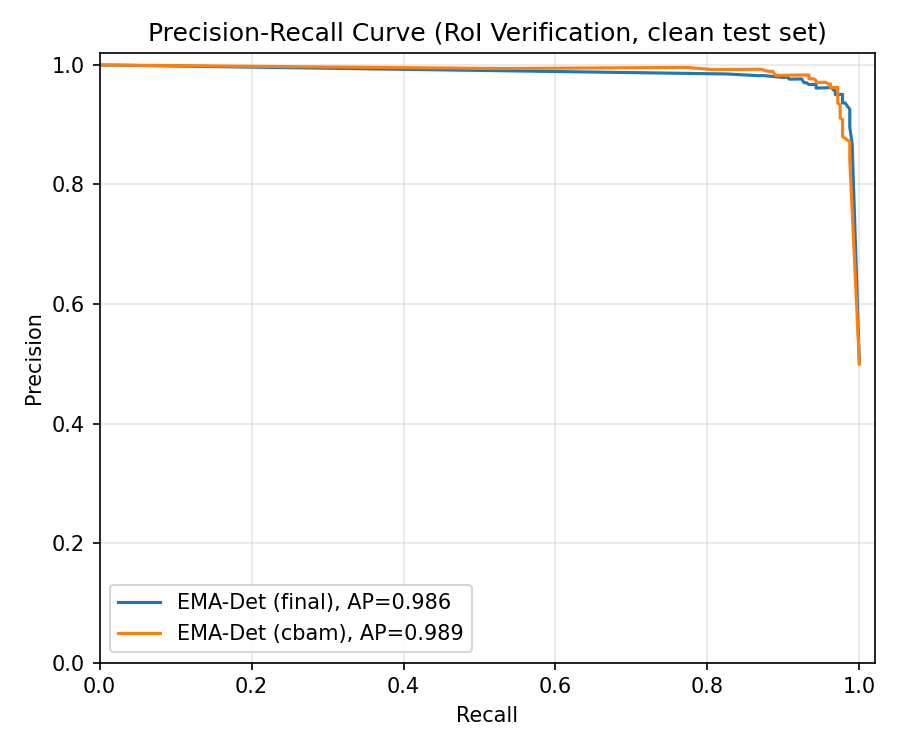
\includegraphics[width=0.6\textwidth]{../results/pr_curve.png}
\caption{Precision-recall curves, clean test set.}
\label{fig:pr}
\end{figure}

\subsection{Hardware Validation Status}
\label{sec:hardware}

\textbf{This section reports only what has actually been measured or
built; no synthesis numbers are fabricated or estimated.} Both trained
configurations were exported to ONNX and verified bit-for-bit-close against
the PyTorch model (max abs.\ difference $<2\times10^{-5}$ over 20 random
inputs). On the development machine (RTX~4060 laptop GPU + host CPU — not
Jetson/FPGA), single-sample PyTorch-CUDA inference reaches 465.0 FPS
(final) / 262.6 FPS (CBAM); ONNX Runtime's CPU execution provider reaches
1018.9 / 650.1 FPS respectively (this development environment's
onnxruntime-gpu build could not load its CUDA/TensorRT provider libraries —
a local dependency issue, not a claim about GPU-accelerated ONNX
performance in general).

A literal C++ translation of the Block1$\to$Gate1$\to$Block4$\to$Gate2
path, using the actual trained (BatchNorm-folded) weights and a testbench
validating it against PyTorch reference outputs on real test images, has
been prepared for Vivado/Vitis HLS synthesis targeting a Zynq-7020 (see
\texttt{hardware/}). \textbf{It has not been compiled, simulated, or
synthesized} — this development environment has no C/C++ toolchain and no
Vivado/Vitis HLS installation. LUT, BRAM, latency, and power figures
require running the prepared \texttt{run\_hls.tcl} flow on a machine with
the toolchain, plus resolving a known design gap (current per-layer buffer
sizing exceeds the Zynq-7020's on-chip BRAM budget; an AXI4-Stream/
line-buffer restructuring is planned, informed by real \texttt{csynth}
resource reports rather than estimated in advance). \emph{We report this
status transparently rather than presenting placeholder numbers as
measurements.}


\section{Limitations}
\begin{itemize}
\item \textbf{Dataset size.} Deduplication reduced the corrected dataset to
4{,}136 patches (from 23{,}620 pre-deduplication) — a much smaller training
set than the conference version used, which may itself limit both absolute
performance and how tightly seed variance can be controlled. Expanding the
raw source pool with additional, verified-non-duplicate UAV photography is
future work.
\item \textbf{Cross-sensor generalization.} The original research plan
included evaluating EO/thermal-IR generalization; no thermal UAV dataset
was available at the time of this draft, and this claim is not made here.
\item \textbf{Hardware validation.} See Section~\ref{sec:hardware} — FPGA
synthesis is prepared but not executed in this draft.
\end{itemize}


\section{Conclusion}
This extended version corrects two methodological issues in our conference
report — a CBAM/training-budget confound and a train/test leakage bug
traced to undeduplicated, patch-level-split source photographs — and
re-establishes EMA-Det's results under a controlled, $N=5$-seed protocol on
a verified leakage-free dataset. The corrected picture is more nuanced than
originally reported: CBAM is not uniformly harmful to this architecture, but
introduces recall instability across training runs severe enough to
disqualify it from a reliability-sensitive edge deployment. We view
publishing this correction, together with the tooling that found it
(\texttt{check\_leakage.py}, \texttt{check\_raw\_duplicates.py}), as itself
a contribution for others building similar two-stage RoI-verification
datasets from web-aggregated source imagery.


\bibliographystyle{plain}
\bibliography{refs}

\end{document}
